\documentclass[tikz,border=8pt]{standalone}
\usepackage{pgfplots}
\pgfplotsset{compat=1.18}
\definecolor{chapterteal}{HTML}{196F6B}
\definecolor{chapterrust}{HTML}{A3472F}
\definecolor{chaptergold}{HTML}{C58B18}
\definecolor{chapterblue}{HTML}{174F75}

\begin{document}

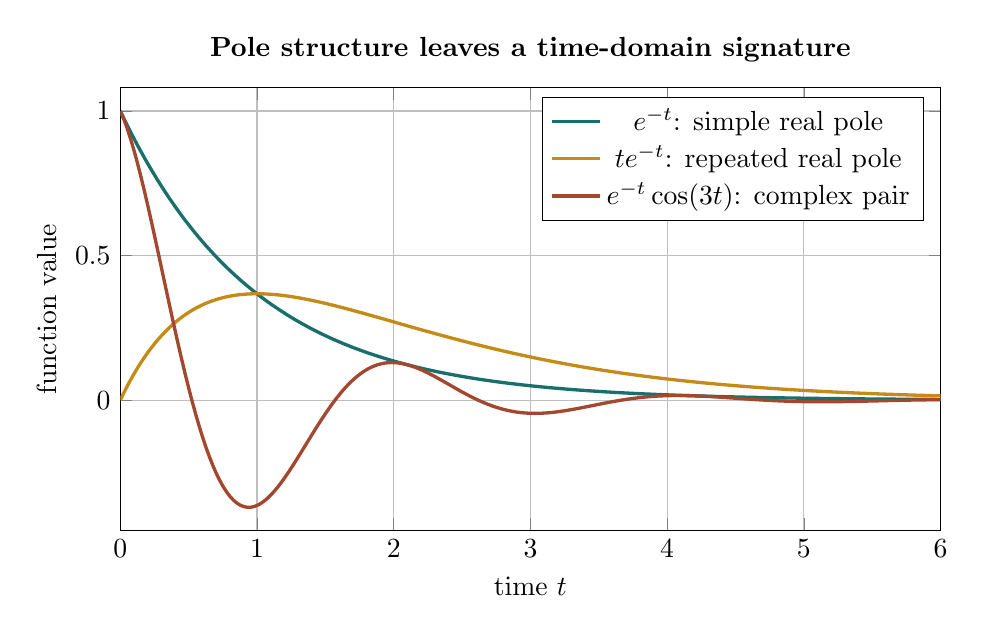
\begin{tikzpicture}
\begin{axis}[
  width=12cm,
  height=7.2cm,
  xmin=0,xmax=6,
  ymin=-0.45,ymax=1.08,
  xlabel={time $t$},
  ylabel={function value},
  title={Pole structure leaves a time-domain signature},
  title style={font=\bfseries},
  grid=both,
  legend style={at={(0.98,0.98)},anchor=north east},
  samples=240,
  domain=0:6
]
\addplot[chapterteal,very thick] {exp(-x)};
\addlegendentry{$e^{-t}$: simple real pole}
\addplot[chaptergold,very thick] {x*exp(-x)};
\addlegendentry{$te^{-t}$: repeated real pole}
\addplot[chapterrust,very thick] {exp(-x)*cos(deg(3*x))};
\addlegendentry{$e^{-t}\cos(3t)$: complex pair}
\end{axis}
\end{tikzpicture}

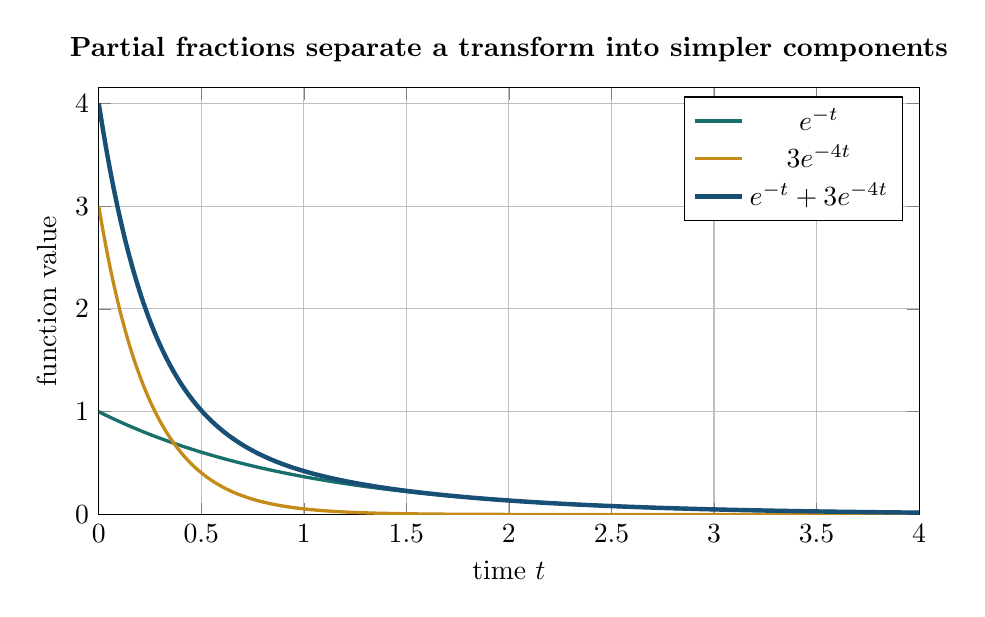
\begin{tikzpicture}
\begin{axis}[
  width=12cm,
  height=7cm,
  xmin=0,xmax=4,
  ymin=0,ymax=4.15,
  xlabel={time $t$},
  ylabel={function value},
  title={Partial fractions separate a transform into simpler components},
  title style={font=\bfseries},
  grid=both,
  legend style={at={(0.98,0.98)},anchor=north east},
  samples=220,
  domain=0:4
]
\addplot[chapterteal,very thick] {exp(-x)};
\addlegendentry{$e^{-t}$}
\addplot[chaptergold,very thick] {3*exp(-4*x)};
\addlegendentry{$3e^{-4t}$}
\addplot[chapterblue,ultra thick] {exp(-x)+3*exp(-4*x)};
\addlegendentry{$e^{-t}+3e^{-4t}$}
\end{axis}
\end{tikzpicture}

\end{document}
